\scanpage{281}
\[
\begin{array}{ll}
M\otimes s\otimes M'\otimes s & M\otimes M'\otimes s\otimes s\\
\mathrm{id}_M\otimes u_s\otimes\mathrm{id}_{M'}\otimes\mathrm{id}_s & \mathrm{id}_{\unsure{M'}}\otimes u_s\otimes\mathrm{id}_s\\
\mathrm{id}_M\otimes\mathrm{id}_s\otimes\mathrm{id}_{M'}\otimes u_s & \mathrm{id}_{\unsure{M'}}\otimes\mathrm{id}_s\otimes u_s
\end{array}
\]
\[
s\boxtimes s=s\qquad s\boxtimes C\simeq C
\]
\margin{\(\unsure{s\perp}\)}
\[
\boxed{(M\otimes_k s)\boxtimes_s C\simeq M\otimes_k C}\qquad ?
\]
\margin{NON\quad\(\odot\)}
\diagram{\begin{tikzcd}
(M\otimes_k\overbrace{s)\otimes_k C}) & M\otimes_k C\arrow[l]
\end{tikzcd}}
\[
\mathrm{id}_M\otimes u_s\otimes\mathrm{id}_C
\qquad
\mathrm{id}_M\otimes\mathrm{id}_s\otimes u_C
\]
\diagram{\begin{tikzcd}
C\arrow[r] & C\otimes_k s\arrow[r,shift left=.5ex]\arrow[r,shift right=.5ex] & C\otimes_k s\otimes_k s
\end{tikzcd}}
\deleted{\(V(s)\otimes V(C)\longrightarrow V(C')\quad\unsure{V(}\)}
\[
\operatorname{Hom}_k(M,s^{k'})\times C^{k'}\longrightarrow C'^{k'}
\]
\margin{\(V(M\otimes_k s)^{k'}=\operatorname{Hom}_k(M.\)}
\deleted{\(\unsure{M}\)}
\[
\operatorname{Hom}_{\unsure{k|k'}}(M\otimes_k s,k')=\operatorname{Hom}_k(M,s^{k'})
\quad\text{est un }s^{\unsure{k|k'}}\text{-module !}
\]
\deleted{
\[
\alpha_*(\unsure{M}),\quad\gamma_0^{(i)}
\]
\[
\Delta\gamma_0^i=\sum_{j+h=i}\gamma_0^j\otimes\gamma_0^h
\]
\[
\beta(\unsure{M})=\sum t^{(i)}\gamma_0^i=\exp(t\gamma_0)
\]
\figure{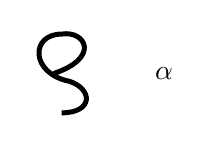
\begin{tikzpicture}[x=1cm,y=1cm]
\draw[line width=1.8pt] (0,.1) .. controls (.6,.3) and (.4,.65) .. (.1,.6) .. controls (-.3,.6) and (-.3,.1) .. (.2,0) .. controls (.5,-.1) and (.5,-.4) .. (.1,-.4);
\node at (1.4,.1) {$\unsure{\alpha}$};
\end{tikzpicture}}
\diagram{\begin{tikzcd}
\widehat A\widehat\otimes\widehat A & \widehat A\arrow[l]
\end{tikzcd}}
\[
\boxed{(\widehat A(\Sigma,\Sigma_+,t))^{k'}=\widehat A_*(\Sigma^{k'},\Sigma_+^{k'},t^{k'})}
\]
\[
\widehat A_*(S,S_+,t)
\]
\[
(A^*(\Sigma,\Sigma_+,t))^\vee=\widehat A_*(\Sigma^\vee,\Sigma_+^\vee,t^\vee)
\]
\figure{\begin{tikzpicture}[x=1cm,y=1cm]
\draw (-4,1.3) .. controls (-5,1) and (-5,-1.2) .. (-3.8,-1.6) .. controls (-1,-2) and (3.8,-1.8) .. (4.3,-.9) .. controls (4.8,.6) and (4.3,1.5) .. (2.9,1.6) .. controls (.4,1.9) and (-3,1.7) .. (-4,1.3);
\node at (-3.7,1.8) {$\Sigma/k$};
\node at (-4.9,.7) {$\deleted{\unsure{R}}$};
\node at (-3.7,.15) {$\begin{array}{c}\Sigma^{\unsure{k'}}\\\bigcup\\\deleted{k}\\\Sigma'\end{array}$};
\draw (-2.9,1.1)--(-2.9,-1.2);
\node[align=left] at (.6,.8) {\(\text{(coalgèbre }\deleted{\unsure{graduée}}\inserted{\unsure{donnée|divisée}}\text{ avec sous-coalgèbre}\)};
\node[align=left] at (.6,.2) {et \unsure{copuiss. divisées} \uline{\unsure{respect celle-ci}}};
\node[align=left] at (.6,-.45) {\unsure{enfin on donne}\quad\(\Sigma\xrightarrow{t}k\)};
\node[align=left] at (.1,-1) {nulle sur \(\deleted{\unsure{k}}\Sigma'\)};
\end{tikzpicture}}
\diagram{\begin{tikzcd}
& t_k\arrow[d,phantom,"{\rotatebox{-90}{\(\unsure{\in|\simeq}\)}}" description] &&\\
0\arrow[r] & \boxed{\unsure{\mathbb Z|Z}}^{k+}\arrow[r] & \underbrace{\Sigma^k}_{\unsure{\text{anneau}}}\arrow[r,nohead] & \Sigma'{}^k\\
& \text{idéal} && \unsure{\text{anneau}}
\end{tikzcd}}
\[
k\{\{T\}\}\{\{\gamma_0,-\gamma_-\}\}
\]
}
\mspage{281}
